\documentclass[a4paper,12pt]{article}

%%% Работа с русским языком
\usepackage{cmap}					% поиск в PDF
\usepackage{mathtext} 				% русские буквы в формулах
\usepackage[T2A]{fontenc}			% кодировка
\usepackage[utf8]{inputenc}			% кодировка исходного текста
\usepackage[english,russian]{babel}	% локализация и переносы
\usepackage{xcolor}
\usepackage{hyperref}
 % Цвета для гиперссылок
\definecolor{linkcolor}{HTML}{799B03} % цвет ссылок
\definecolor{urlcolor}{HTML}{799B03} % цвет гиперссылок

\hypersetup{pdfstartview=FitH,  linkcolor=linkcolor,urlcolor=urlcolor, colorlinks=true}

%%% Дополнительная работа с математикой
\usepackage{amsfonts,amssymb,amsthm,mathtools} % AMS
\usepackage{amsmath}
\usepackage{icomma} % "Умная" запятая: $0,2$ --- число, $0, 2$ --- перечисление

%% Номера формул
%\mathtoolsset{showonlyrefs=true} % Показывать номера только у тех формул, на которые есть \eqref{} в тексте.

%% Шрифты
\usepackage{euscript}	 % Шрифт Евклид
\usepackage{mathrsfs} % Красивый матшрифт

%% Свои команды
\DeclareMathOperator{\sgn}{\mathop{sgn}}

%% Перенос знаков в формулах (по Львовскому)
\newcommand*{\hm}[1]{#1\nobreak\discretionary{}
{\hbox{$\mathsurround=0pt #1$}}{}}
% графика
\usepackage{graphicx}
\graphicspath{{pictures/}}
\DeclareGraphicsExtensions{.pdf,.png,.jpg}
\author{Бурмашев Григорий, БПМИ-208}
\title{}
\date{\today}
\begin{document} 
\begin{center}
Бурмашев Григорий. 208. ИДЗ -- 7

Вариант 2
\end{center}
\section*{Номер 1}
\begin{itemize}
\item 
\begin{center}
Дополните вектор $
v = \frac{1}{9}(2, -8, -3, -2)
$ до ортонормированного базиса в $\mathbb{R}^4$
\end{center}
\end{itemize}

Будем пользоваться методом ортогонализации Грама -- Шмидта. Для этого дополним наш вектор до базиса $\mathbb{R}^4$. Нам подойдут векторы из стандартного базиса:
\[
v_2 = (0, 1, 0, 0)
\]
\[
v_3 = (0, 0, 1, 0)
\]
\[
v_4 = (0, 0, 0, 1)
\]
Очевидно, что такая система векторов будет линейно независимой. 
\[
v = \left(\frac{2}{9}, -\frac{8}{9}, -\frac{1}{3}, -\frac{2}{9} \right)
\]
Теперь идем по методу:
\[
e_1 = v
\]
\[
e_2 = v_2 - \frac{(v_2, e_1)}{(e_1, e_1)} \cdot e_1 = \begin{pmatrix}
0 \\ 1 \\ 0 \\ 0 
\end{pmatrix}
 - \frac{-\frac{8}{9}}{1} \cdot \begin{pmatrix}
\frac{2}{9} \\ -\frac{8}{9} \\-\frac{1}{3} \\ -\frac{2}{9} 
\end{pmatrix} =
\begin{pmatrix}
0 \\ 1 \\ 0 \\ 0 
\end{pmatrix}
 + \frac{8}{9} \cdot \begin{pmatrix}
\frac{2}{9} \\ -\frac{8}{9} \\-\frac{1}{3} \\ -\frac{2}{9} 
\end{pmatrix} =
\]
\[
=
\begin{pmatrix}
0 \\ 1 \\ 0 \\ 0 
\end{pmatrix} + 
\begin{pmatrix}
\frac{16}{81} \\ -\frac{64}{81} \\-\frac{8}{27} \\ -\frac{16}{81} 
\end{pmatrix} = \begin{pmatrix}
\frac{16}{81} \\ \frac{17}{81} \\-\frac{8}{27} \\ -\frac{16}{81} 
\end{pmatrix}
\]
\[
e_3 = v_3 - \frac{(v_3, e_1)}{(e_1, e_1)}  \cdot e_1- \frac{(v_3, e_2)}{(e_2, e_2)} \cdot e_2 = \begin{pmatrix}
0 \\ 0 \\ 1 \\ 0
\end{pmatrix} + \frac{1}{3} \cdot e_1  + \frac{\frac{8}{27}}{\frac{17}{81}} \cdot e_2 = 
\]
\[
=
\begin{pmatrix}
0 \\ 0 \\ 1 \\ 0
\end{pmatrix} + \begin{pmatrix}
\frac{2}{27} \\ -\frac{8}{27} \\-\frac{1}{9} \\ -\frac{2}{27} 
\end{pmatrix} + \frac{24}{17} \cdot \begin{pmatrix}
\frac{16}{81} \\ \frac{17}{81} \\-\frac{8}{27} \\ -\frac{16}{81} 
\end{pmatrix} = \begin{pmatrix}
\frac{2}{27} \\ -\frac{8}{27} \\ \frac{8}{9} \\ -\frac{2}{27} 
\end{pmatrix}  + \begin{pmatrix}
\frac{128}{459} \\ \frac{8}{27} \\-\frac{64}{153} \\ -\frac{128}{459} 
\end{pmatrix}
=
\begin{pmatrix}
\frac{6}{17} \\ 0 \\ \frac{8}{17} \\ -\frac{6}{17}
\end{pmatrix}
\]
\clearpage
\[
e_4 = v_4 - \frac{(v_4, e_1)}{(e_1, e_1)} \cdot e_1 -  \frac{(v_4, e_2)}{(e_2, e_2)} \cdot e_2  -\frac{(v_4, e_3)}{(e_3, e_3)} \cdot e_3 = \begin{pmatrix}
0 \\ 0 \\ 0 \\ 1
\end{pmatrix} 
+ \frac{2}{9} \cdot e_1 + \frac{\frac{16}{81}}{\frac{17}{81}}e_2  + \frac{\frac{6}{17}}{\frac{8}{17}} \cdot e_3 =
\]
\[
=
\begin{pmatrix}
0 \\ 0 \\ 0 \\ 1
\end{pmatrix}  + \begin{pmatrix}
\frac{4}{81} \\ -\frac{16}{81} \\ -\frac{2}{27} \\ -\frac{4}{81}
\end{pmatrix}
+ \frac{16}{17} \cdot \begin{pmatrix}
\frac{16}{81} \\ \frac{17}{81} \\-\frac{8}{27} \\ -\frac{16}{81} 
\end{pmatrix} + \frac{3}{4} \cdot \begin{pmatrix}
\frac{6}{17} \\ 0 \\ \frac{8}{17} \\ -\frac{6}{17}
\end{pmatrix} = \begin{pmatrix}
\frac{4}{81} \\ -\frac{16}{81} \\ -\frac{2}{27} \\ \frac{77}{81}
\end{pmatrix} + \begin{pmatrix}
\frac{256}{1377} \\ \frac{16}{81} \\ -\frac{128}{459} \\ -\frac{256}{1377}
\end{pmatrix}
+
\begin{pmatrix}
\frac{9}{34} \\ 0 \\ \frac{6}{17} \\ -\frac{9}{34}
\end{pmatrix}
=
\begin{pmatrix}
\frac{1}{2} \\ 0 \\ 0 \\ \frac{1}{2}
\end{pmatrix}
\]
Получили векторы $e_1, e_2, e_3, e_4$. Теперь ортонормируем их:
{\Large \[
f_1 = \frac{e_1}{|e_1|} = \begin{pmatrix}
\frac{2}{9} \\ -\frac{8}{9} \\ -\frac{1}{3} \\ -\frac{2}{9}
\end{pmatrix}
\]
\[
f_2 = \frac{e_2}{|e_2|} = \frac{9}{\sqrt{17}} \cdot e_2 = \begin{pmatrix}
\frac{16}{9 \sqrt{17}} \\ \frac{\sqrt{17}}{9} \\ - \frac{8}{3\sqrt{17}} \\ -\frac{16}{9 \sqrt{17}}
\end{pmatrix}
\]
\[
f_3 = \frac{e_3}{|e_3|} = \frac{1}{\sqrt{\frac{8}{17}}} \cdot 
\begin{pmatrix}
\frac{6}{17} \\ 0 \\ \frac{8}{17} \\ -\frac{6}{17}
\end{pmatrix}
\]
\[
f_4 = \frac{e_4}{|e_4|} = \frac{1}{\sqrt{\frac{1}{2}}} \cdot \begin{pmatrix}
\frac{1}{2} \\ 0 \\ 0 \\ \frac{1}{2}
\end{pmatrix} 
\]}
\begin{center}
\textbf{Ответ: } дополнили векторами $f_2, f_3, f_4$
\end{center}
\clearpage

\section*{Номер 2}
\begin{itemize}
\item
\begin{center}
Подпространство $U$ евклидова пространства $\mathbb{R}^4$ задано системой уравнений:
\[
\begin{cases}
-x_1 + 6x_2 - 7x_3 + 5x_4 = 0 \\
2x_1 - 7x_2 + 9x_3 - 5x_4 = 0
\end{cases}
\]
Для вектора $v = (0, 1, -1, -2)$ найдите его проекцию на $U$, его ортогональную составляющую относительно $U$ и расстояние от него до $U$.
\end{center}
\end{itemize}
Находим базис $U$:
\[
\begin{pmatrix}
-1 & 6 & -7 & 5 & \\
2 & -7 & 9 & -5 & \\
\end{pmatrix}
=
\begin{pmatrix}
-1 & 6 & -7 & 5 & \\
0 & 5 & -5 & 5 & \\
\end{pmatrix}
=
\]
\[
=
\begin{pmatrix}
-1 & 0 & -1 & -1 & \\
0 & 1 & -1 & 1 & \\
\end{pmatrix}
=
\begin{pmatrix}
1 & 0 & 1 & 1 & \\
0 & 1 & -1 & 1 & \\
\end{pmatrix}
\]
Тогда ФСР имеет вид:
\[
f_1 = 
\begin{pmatrix}
-1 \\ 1 \\ 1 \\ 0
\end{pmatrix}, 
f_2 =
\begin{pmatrix}
-1 \\ -1 \\ 0 \\ 1
\end{pmatrix}
\]
$(f_1, f_2) = 0$. Тогда:
\[
\text{pr}_u v = \frac{(v, f_1)}{(f_1, f_1)}f_1 + \frac{(v, f_2)}{(f_2, f_2)}f_2 = \frac{0}{3}f_1 + \frac{-3}{3}f_2 = \begin{pmatrix}
1 \\ 1 \\ 0 \\ -1
\end{pmatrix}
\]
Из формулы $v = \text{pr}_u v + \text{ort}_u v$ получаем:
\[
\text{ort}_u v = v - \text{pr}_u v  = \begin{pmatrix}
0 \\ 1 \\ -1 \\ -2
\end{pmatrix}
 - \begin{pmatrix}
1 \\ 1 \\ 0 \\ -1
\end{pmatrix}
= 
\begin{pmatrix}
-1 \\ 0 \\ -1 \\ -1
\end{pmatrix}
\]
Теперь находим расстояние:
\[
p(v, u) = |\text{ort}_u v| = \sqrt{3} 
\]
{\Large \begin{center}
\textbf{Ответ: } 
\[
\text{pr}_u v = \begin{pmatrix}
1 \\ 1 \\ 0 \\ -1
\end{pmatrix}
\]
\[
\text{ort}_u v = \begin{pmatrix}
-1 \\ 0 \\ -1 \\ -1
\end{pmatrix}
\]
\[
p(v, u) = \sqrt{3} 
\]
\end{center}}
\clearpage

\section*{Номер 3}
\begin{itemize}
\item
\begin{center}
Составьте уравнение прямой в $\mathbb{R}^3$, параллельной плоскости $x - y - 5z = 3$, проходящей через точку $(8, -6, 2)$ и пересекающей прямую $x = 3t, y = -4t + 5, z = 2t-3$
\end{center}
\end{itemize}
Введем названия для удобства:
\[
l \text{ -- искомая прямая}
\]
\[
l_0 \text{ -- прямая, которую пересекает } l
\]
\[
\alpha \text{ -- плоскость} 
\]
\[
M \text{ -- точка } (8, -6, 2)
\]
Нормаль плоскости $\alpha$ будет : $(1, -1, -5)$
\\\\
Составим нашу прямую, которая проходит через точку $M$:
\[
l = \begin{pmatrix}
x \\ y \\ z
\end{pmatrix}p + \begin{pmatrix}
8 \\ -6 \\ 2
\end{pmatrix}
\]
По условию $l \; ||  \; \alpha$, следовательно $(l, (1, -1, -5)) = 0$, т.е:
\[
x - y - 5z = 0
\]
\[
x = y + 5z
\]
Тогда можем найти коэффы для прямой:
\[
l = \begin{pmatrix}
y+ 5z \\ y\\ z
\end{pmatrix}p + \begin{pmatrix}
8 \\ -6 \\ 2
\end{pmatrix}
\]
Прямая пересекает прямую $l_0$, приравняем их координаты:
\[
\begin{cases}
yp + 5zp +8 = 3t \\
yp -6 = -4t + 5\\
zp +2 = 2t - 3
\end{cases}
\]
\[
\begin{cases}
yp + 5zp +8 = 3t \\
yp  = -4t + 11\\
zp  = 2t - 5
\end{cases}
\]
Отсюда:
\[
\begin{cases}
t = 2\\
yp = 3\\
z p = -1\\
xp = yp + 5zp = 3 - 5 = -2 
\end{cases}
\]
Тогда получаем, что:
\[
l = \begin{pmatrix}
-2 \\ 3 \\ -1 
\end{pmatrix}p + \begin{pmatrix}
8 \\ -6 \\ 2
\end{pmatrix}
\]
{\Large \begin{center}
\textbf{Ответ: } 
\[
l = \begin{pmatrix}
-2 \\ 3 \\ -1 \\
\end{pmatrix}p + \begin{pmatrix}
8 \\ -6 \\ 2 \\
\end{pmatrix}
\]
\end{center}}
\clearpage
\section*{Номер 4}
\begin{itemize}
\item
\begin{center}
Дан куб $ABCDA'B'C'D'$ со стороной 14. Точка $F$ -- середина ребра $BB'$, а точка $E$ лежит на ребре $BB'$, причём $BE : EB' = 4 : 3$. Найдите угол и расстояние между прямой $AE$ и $D'F$
\end{center}
\end{itemize}

\begin{center}
{\Large График:}
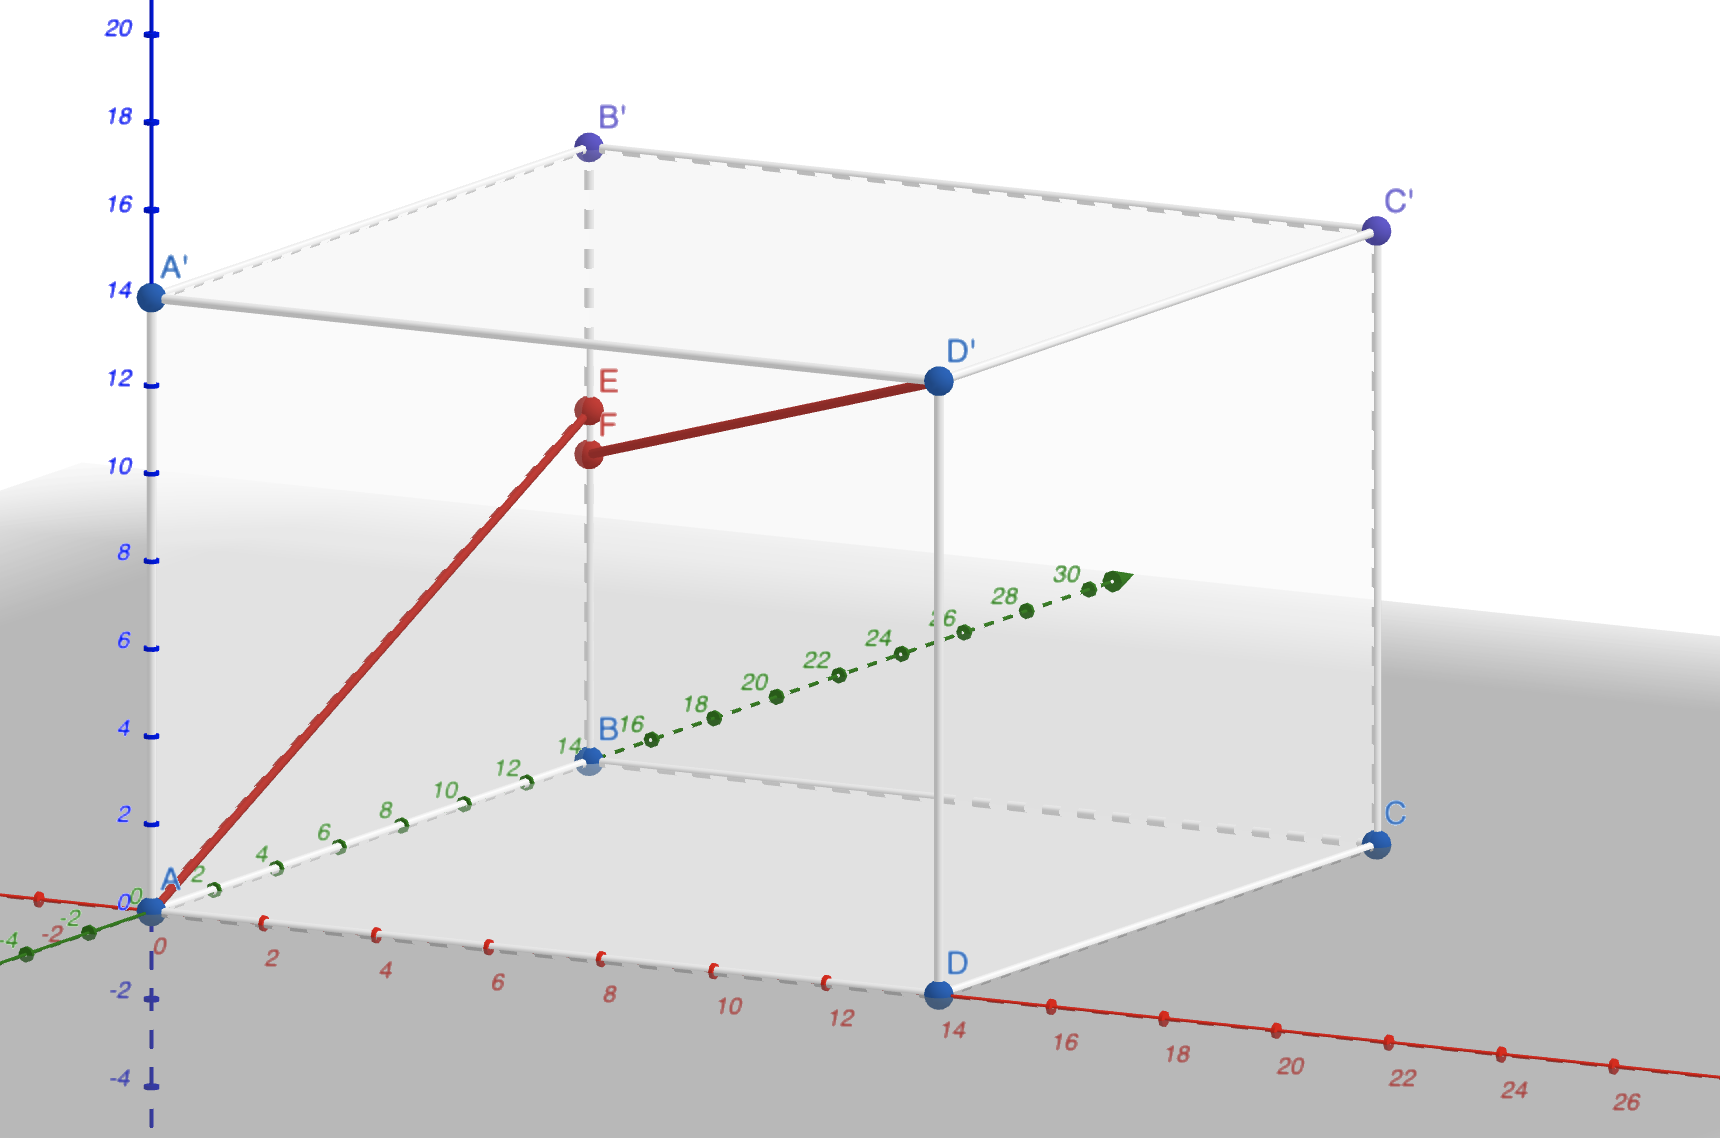
\includegraphics[scale=0.4]{4.png}
\end{center}
\begin{center}
{\Large Условие:}

$AB = 14, BE : EB' = 4:3$

Пусть  A -- начало координат, AD задает ось x, AB задает ось y, AA' задает ось z.

Тогда координаты точек:
\end{center}
$
A(0, 0, 0), \;
$
$
B'(0, 14, 14),\;
$
$
D'(14, 0, 14), \;
$
$
F(0, 14, 7), \;
$
$
E(0, 14, 8)
$
\\\\
Тогда:
\[
\overrightarrow{AE} = (0, 14, 8)
\]
\[
\overrightarrow{D'F} = (-14, 14, -7)
\]
\[
\overrightarrow{EF} = (0, 0, -1)
\]
Теперь считаем угол (по формуле с лекций):
\[
\cos \phi = \frac{|(\overrightarrow{AE}, \overrightarrow{D'F})|}{|\overrightarrow{AE}| \cdot |\overrightarrow{D'F}| } = \frac{140}{\sqrt{260} \cdot \sqrt{441}} = \frac{2 \sqrt{65}}{39}
\]
\[
\phi = \arccos \left( \frac{2 \sqrt{65}}{39} \right)
\]
Cчитаем расстояние (также по ст.формуле):
\[
p(AE, D'F) = \frac{|\left(AE, D'F, EF\right)|}{|\left[AE, D'F\right]|} = \frac{|\left(\left[AE, D'F\right], EF\right)|}{|\left[AE, D'F\right]|} 
\]
Отдельно посчитаем:
\[
\left[AE, D'F\right] = \begin{vmatrix}
e_1 & e_2 & e_3 \\
0 & 14 & 8 \\
-14 & 14 & -7 
\end{vmatrix} = 
\]
\[
=
e_1 \cdot \begin{vmatrix}
14 & 8 \\14 & -7
\end{vmatrix}  - e_2 \cdot  \begin{vmatrix}
0 & 8 \\-14 & -7
\end{vmatrix} + e_3 \cdot \begin{vmatrix}
0 & 14 \\
-14 & 14
\end{vmatrix} = -210 \cdot e_1  - 112 \cdot e_2 \cdot + 196 \cdot e_3 = 
\]
\[
=
\begin{pmatrix}
-210 \\ -112 \\ 196
\end{pmatrix}
\]
\[
|[AE, D'F]| = 14 \sqrt{485}
\]
\[
|\left(\left[AE, D'F\right], EF\right)| = -196
\]
Возвращаемся к расстоянию:
\[
p(AE, D'F) = 
-\frac{196}{14\sqrt{485}} = - \frac{14}{\sqrt{485}}
\]
{\Large \begin{center}
\textbf{Ответ: } 
\[
\angle = \arccos \left( \frac{2 \sqrt{65}}{39} \right)
\]
\[
p(AE, D'F) =  - \frac{14}{\sqrt{485}}
\]
\end{center}}
\end{document}
